\section{Polygonal Meshes}
\label{sec:polygonal}

In this section, we introduce polygonal meshes, describe a data structure to 
work with them, and introduce the Euler characteristic of a mesh.

\subsection{What is a surface?}

Most solid objects in our world have boundaries that are surfaces.
Often, it is useful to represent a these boundary surfaces using computers.
Examples of representing surfaces include computer graphics and modeling solids for manufacturing.
Surfaces can be represented by connecting polygons together, we call these building blocks
vertices, edges, and faces. We denote the set of vertices, edges and faces in a surface as 
$V, E$ and $F$ respectively. We call such a surface a \emph{mesh}
or triangulated mesh, if all faces are triangles.
An example of a triangular mesh is shown in \figref{cat},
notice that this mesh has a boundary on the collar, eyes, and mouth.
Let $\partial(V)$ denote vertices on the boundary of a surface and let $V_{int}$ 
denote vertices that are not on the boundary.
One question we must face when representing smooth surfaces as a polygonal mesh is:
how many faces do we need in order for the surface to not appear faceted?
More small triangles we give us a better approximation but we pay a price in computational
efficiency. 



 \begin{figure}[htb]
         \centering
        \begin{subfigure}[b]{0.3\textwidth}
         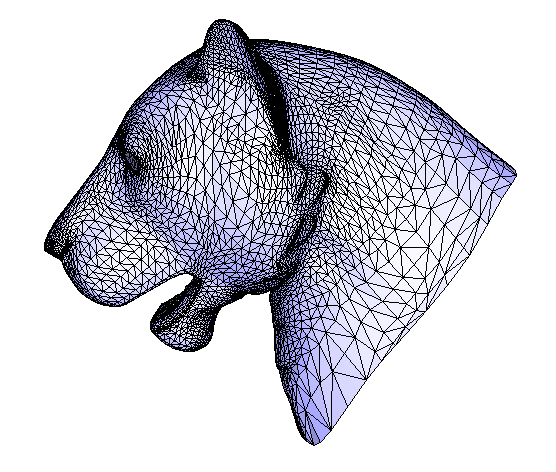
\includegraphics[width=\textwidth]{polygonal-mesh/profile}
         \caption{}
 	 \label{fig:profile}
       \end{subfigure}
         \hspace{.6cm}
         \begin{subfigure}[b]{0.19\textwidth}
         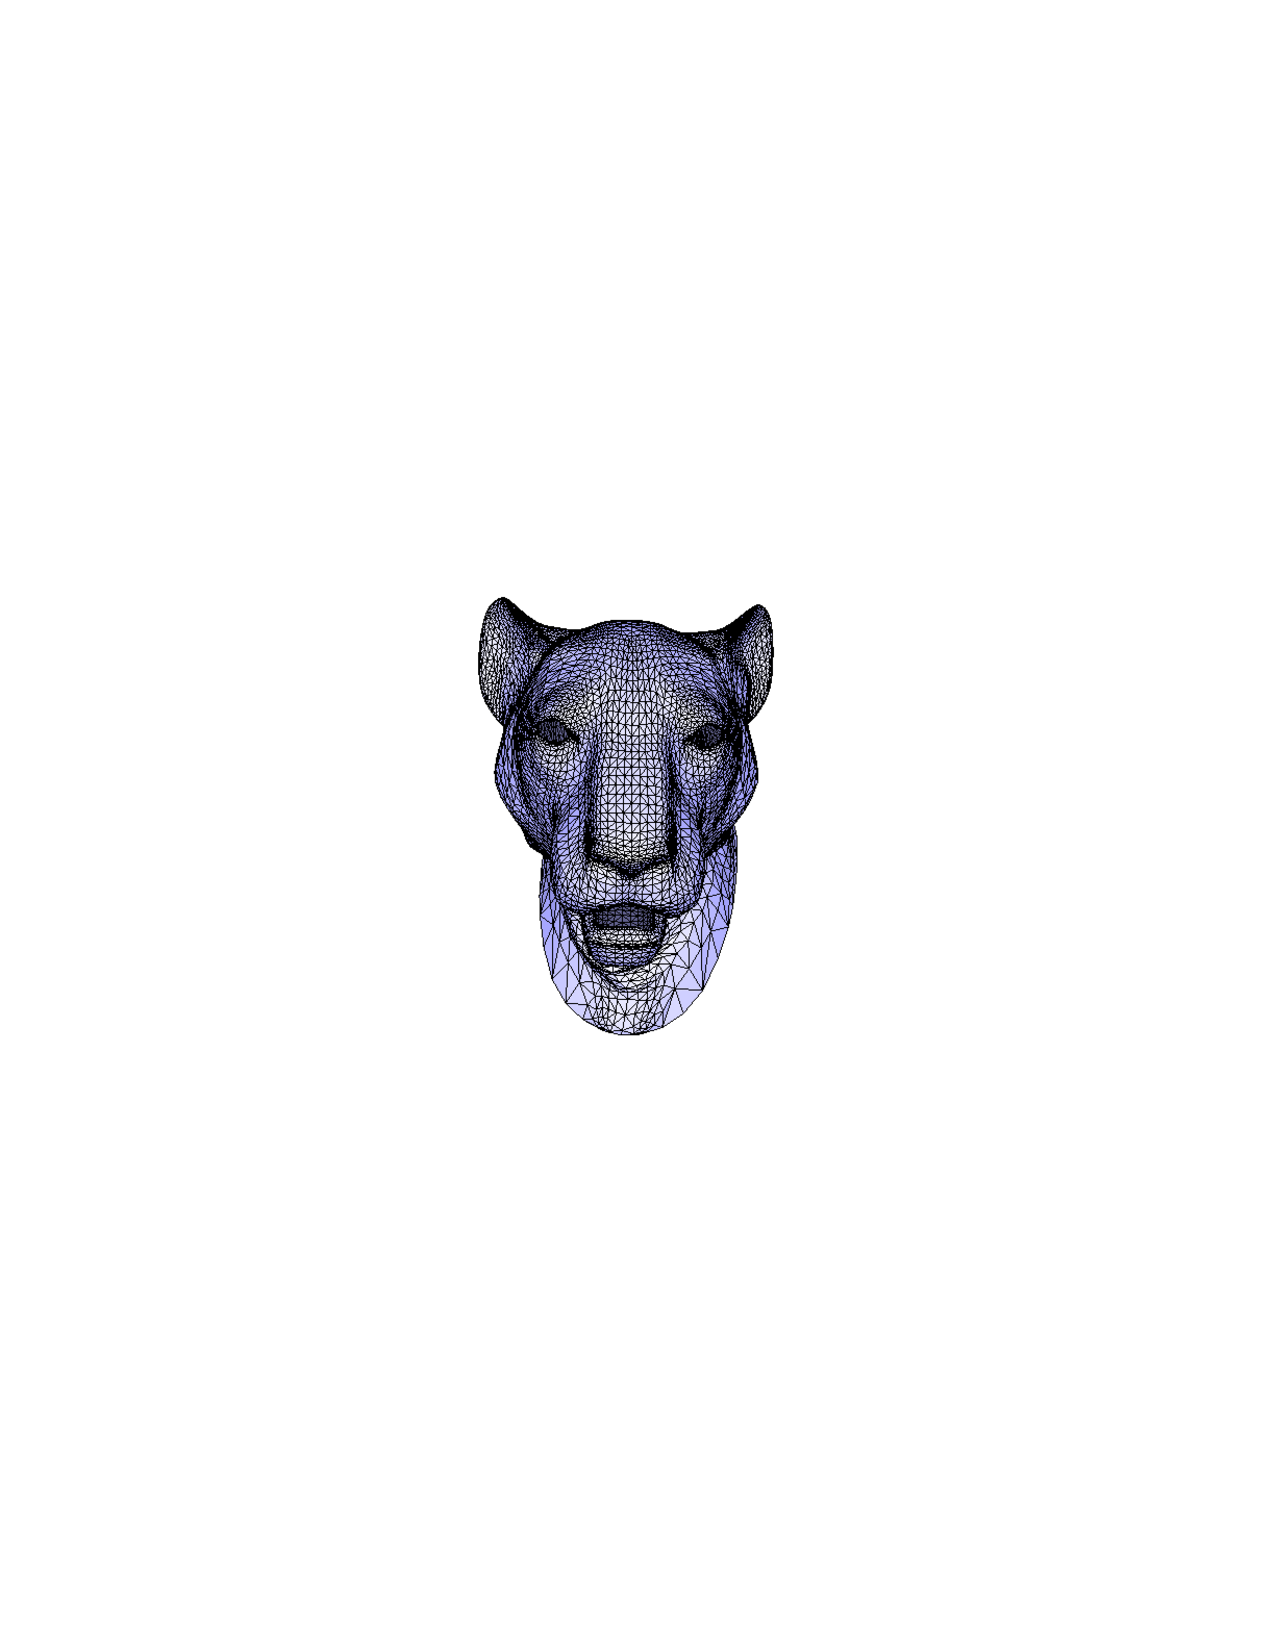
\includegraphics[width=\textwidth]{polygonal-mesh/head-on}
         \caption{}
          \label{fig:head-on}
         \end{subfigure}
             \hspace{.6cm}
         \begin{subfigure}[b]{0.24\textwidth}
         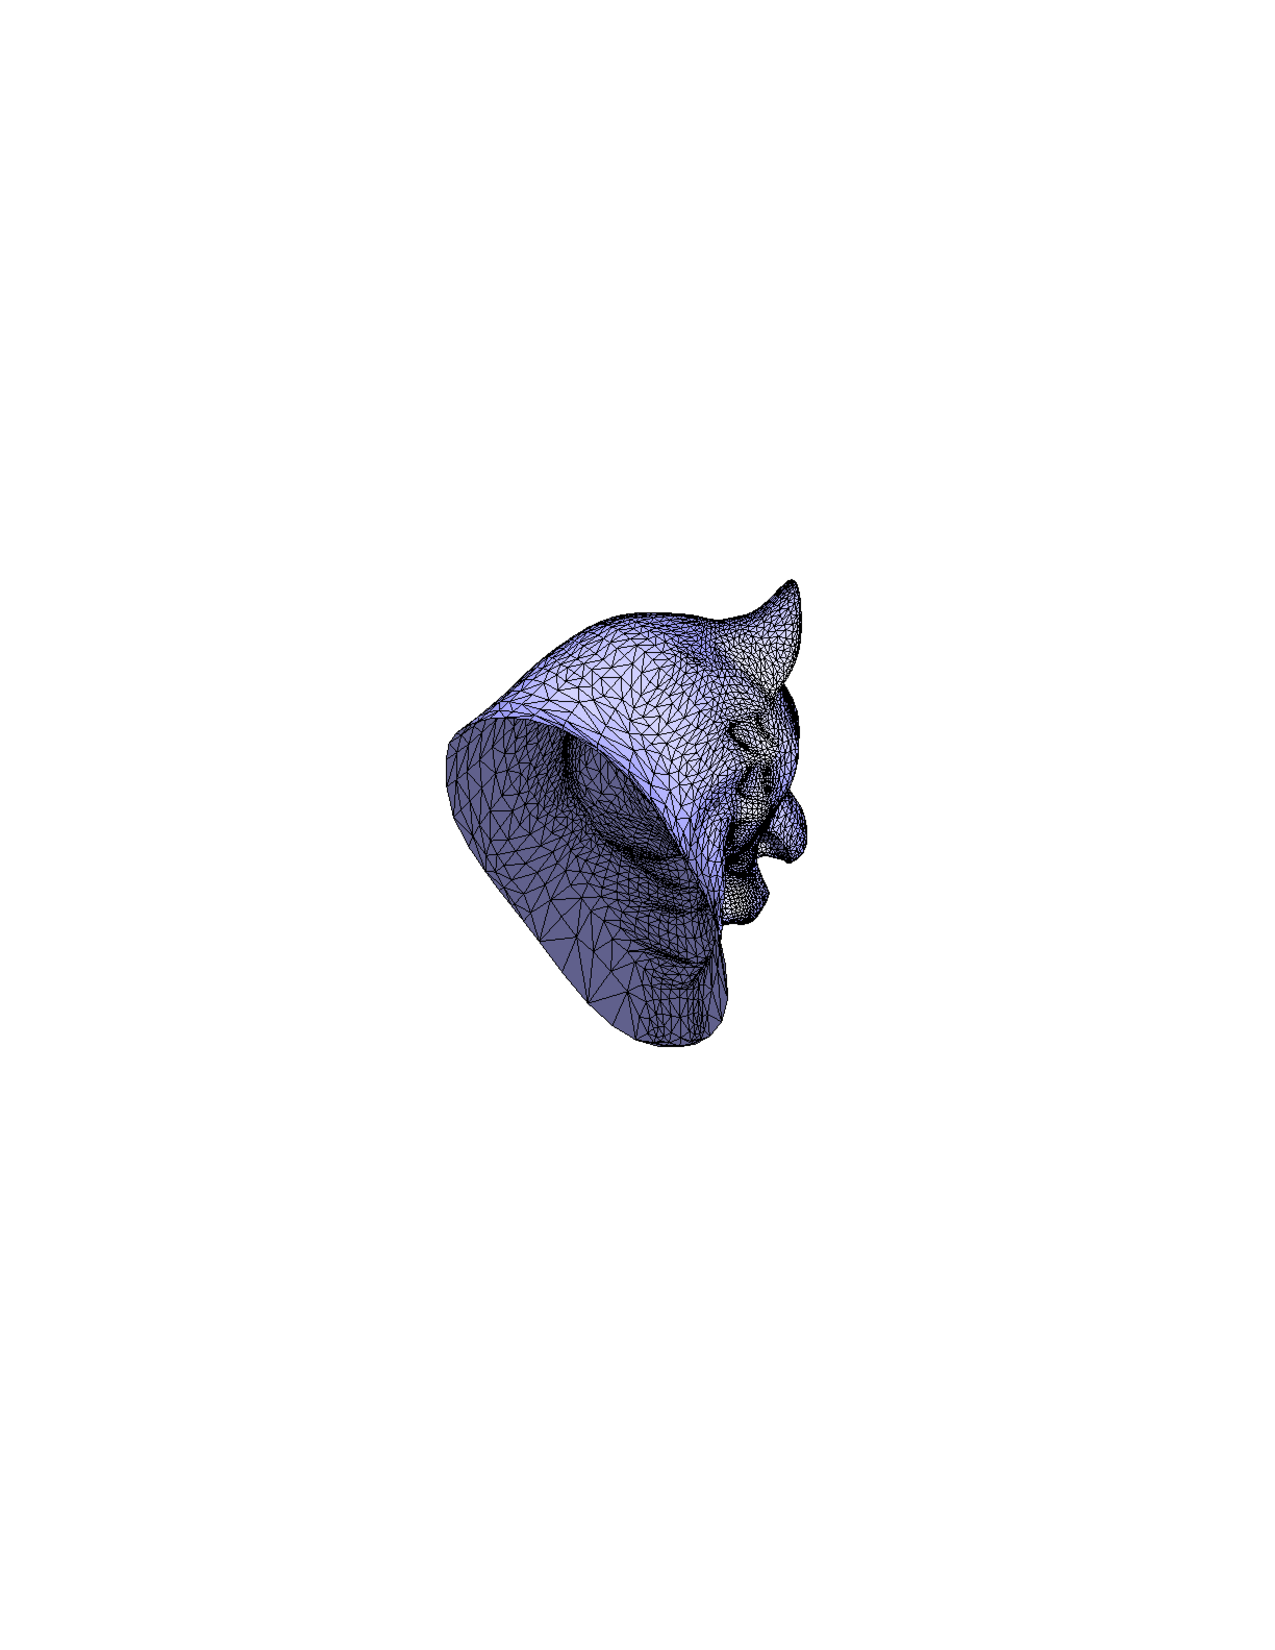
\includegraphics[width=\textwidth]{polygonal-mesh/back}
         \caption{}
          \label{fig:back}
         \end{subfigure}
		\caption{(\subref{fig:profile}) A profile view of a mesh.
 		(\subref{fig:head-on})  A frontal view of the same mesh and the view from the back (\subref{fig:back}).
 		\label{fig:cat}}
 \end{figure}

One way to store a mesh in a computer is as a OFF file.
The first optional line of an OFF file identifies the file as an OFF file.
The second line lists the number of vertices, faces, and edges.
A list of vertices in $(x,y,z)$ coordinates is then given followed
by a list of faces indicated by the index of the vertices contained in the face.
For the mesh in \figref{cat}, the OFF file looks is shown in 
\tabref{off}.

\begin{table}[h!]
\caption{The OFF data for the mesh in \figref{cat}.}
\centering
\begin{tabular}{|p{2cm} p{2cm} p{2cm} p{2cm}|} 
 \hline
\texttt{OFF} &  & &  \\ 
\texttt{7529} & \texttt{14859} & \texttt{0} &  \\ 
\texttt{-0.29196} & \texttt{-0.0867173} & \texttt{-0.355149}  &  \\
 \texttt{-0.123586}   & \texttt{-0.0127199} & \texttt{-0.385597} &  \\
\texttt{-0.138255}   & \texttt{-0.0985078} & \texttt{-0.384018} &  \\
  & &\vdots &  \\  
 \texttt{3}&  \texttt{97} &\texttt{1893}& \texttt{1895}\\
 \texttt{3}& \texttt{71} & \texttt{1894} & \texttt{1893} \\
 \texttt{3} & \texttt{16} & \texttt{1895} & \texttt{1894}\\
   & &\vdots &  \\  
 \hline
\end{tabular}

\label{tab:off}
\end{table}

Suppose we work in a machine shop and a customer has an metal object that they would like
to duplicate.
One way to do this, is by 3D scanning the object to capture the coordinates on the 
surface and represent the object as a triangulated mesh, then use a machine to carve the object
from a block of metal. 
While scanning, errors might occur. As a result of these errors
we might obtain a triangulation that intersects itself. If we try to reconstruct the object
from our mesh our machines will have ambiguous information of what the surface of the object
should be.
This motivates developing an algorithm to determine if a mesh has self-intersections.
Determining if two faces intersect using the OFF representation of a surface is combersome.
To simplify algorithms on meshes we load the OFF file into a more convenient data-structure,
the doubly-connected edge list.

\subsection{Doubly-Connected Edge List}

The doubly-connected edge list (DCEL) consists of three separate and related structures, one each
for the vertices, edges, and faces \cite{dutchbook3}.
For each edge, we store two directed half-edges $(\overrightarrow{e})$, with pointers to: its origin, the twin half-edge, the incident face that it bounds, the next half-edge bounding the same face, and the previous half-edge bounding the same face.


For each vertex $v$, we store the coordinates of $v$ and a pointer to an arbitrary half-edge
that has $v$ as its origin.
For each face $f$, we store pointers to an arbitrary half-edge on its boundary. If a face has holes inside of it, we store a list of inner components and pointers to an arbitrary half-edge  on the boundary of each hole.

For the set of vertices, edges, and faces we have iterators that enable us to begin with an arbitrary element
and iterate over all elements. These collections of objects and pointers allow development of
powerful algorithms to work with meshes. An example of a library of meshes algorithms
is the Computational Geometry Library (CGAL) \cite{cgal, cgal:eb-24b}. We will use CGAL algorithms
through out this text.


Back to our motivating example of determining if a mesh intersects itself. 
Assuming our mesh $M$ is given as a DCEL, we can iterate over all pairs of faces
and determine if the faces intersect (how do you determine if two faces intersect?).
Pseudocode for our algorithm is given in \algref{self-intersection}.


\begin{algorithm}
 \caption{Self-intersection}\label{alg:self-intersection}
    \begin{algorithmic}[1]
      \Require A DCEL of a mesh $M.$
        \Ensure A boolean indicating if $M$ has a self-intersection.
        
        \State bool $b=0.$
\For{$f_1\in F$}
	\For{$f_2\in F$}
	
	\If{$f_1\neq f_2\ \&\&\ f_1\cap f_2 \neq \emptyset$} 
		\State $b=1.$
	\EndIf 
	\EndFor
\EndFor
\Return $b$.
\end{algorithmic}
\end{algorithm}



\subsection{The Euler Characteristic}

The \EMPH{Euler characteristic} of a surface triangulated $S$ denoted by $\chi(S)$, or $\chi$
 if the surface is clear,  is the 
the number of vertices minus the number of edges plus  the number of faces, $\chi=|V|-|E|+|F|.$
The Euler characteristic is a topological invariant of a space meaning it
and does not depend on the choice of triangulation.
The Euler characteristic is defined for higher dimensional objects beyond surfaces,
 for a triangulated space $X$ the Euler characteristic is 
$\chi(X)=k_0-k_1+k_2-k_3+\ldots$ where $k_n$ is the number of `triangles' of dimension $n.$



A  graph  is \EMPH{planar} if it can be drawn in the plane with intersections only occurring
at vertices.
Triangulations of the two dimensional sphere $\Sp^2$ and the two dimensional disk $D^2$ 
will be used in our applications.
For the sphere, we have $\chi(\Sp^2)=2$ 
several proofs of this can be found on David Eppstein's website \cite{eppstein-proofs}.




We next give a proof that $\chi(\Sp^2)=2$ due Thurston \cite{thurston}. 
For any planar graph we imagine the graph embedded in the two sphere, by
shrinking the graph until it fits inside of the unit circle, then project the image of the graph
onto the southern hemisphere.  

\begin{theorem}[Euler Characteristic for Planar Graphs]\label{thm:euler}
For any planar graph on the two sphere we have $V-E+F=2.$
\end{theorem}

\begin{proof}
If needed, perturb the triangulation so that the north and south poles are 
inside of  two faces and there are no vertical edges. At each vertex place a unit positive
charge, at the center of each edge place a unit negative charge and put a unit positive
charge in the middle of each face. Slam the sphere on the ground so that all charges
on the edges and vertices are moved into the face below them. For faces that do not contain a pole
the net charge will be zero, the northern boundary consists of an alternating sequence
of edges and vertices  beginning  and ending with an edge.
The face containing the north pole has a unit positive charge, and the face containing the south
pole contains positive four units of charge and negative three units of charge.
Thus, the total charge is two.
\end{proof}

Triangulations of the sphere are a special case of \thmref{euler}.
The sphere will be one of two common surfaces we see in applications
of the Gauss-Bonnet theorem. The other being the disk.
For the disk, $\chi(D^2)=1$. This can be seen by considering
the removal of a single face from a triangulation of the sphere.
Once a face is removed, we can `unwrap' the remaining faces of the sphere
onto the plane to obtain a triangulation of a disk. Moreover, this projection
is invertible and given a triangulation of a disk we can obtain a triangulation
of the sphere with a single face omitted.

The Euler characteristic of a connected, orientable surface surface is often 
stated in terms of the genus of the surface which is defined as follows.
\begin{definition}[Genus of a Surface]\label{def:genus}
	The genus of a connected, orientable surface is the maximum number of
	cuttings along non-intersecting simple closed curves without disconnecting
	the surface \cite{munkres}.
\end{definition}


For an orientable surface, the genus and the Euler characteristic are related by
the formula $\chi=2-2g$. To see this, we can transform a triangulation of a surface of
genus $g$ into a surface of genus $g+1$ by removing two faces and an equal number
of vertices and edges. \figref{genus} provides an example.
Thus, the sphere has genus zero and the torus has genus one.


\begin{figure}[htb]
        \centering
        \begin{subfigure}[b]{0.2\textwidth}
        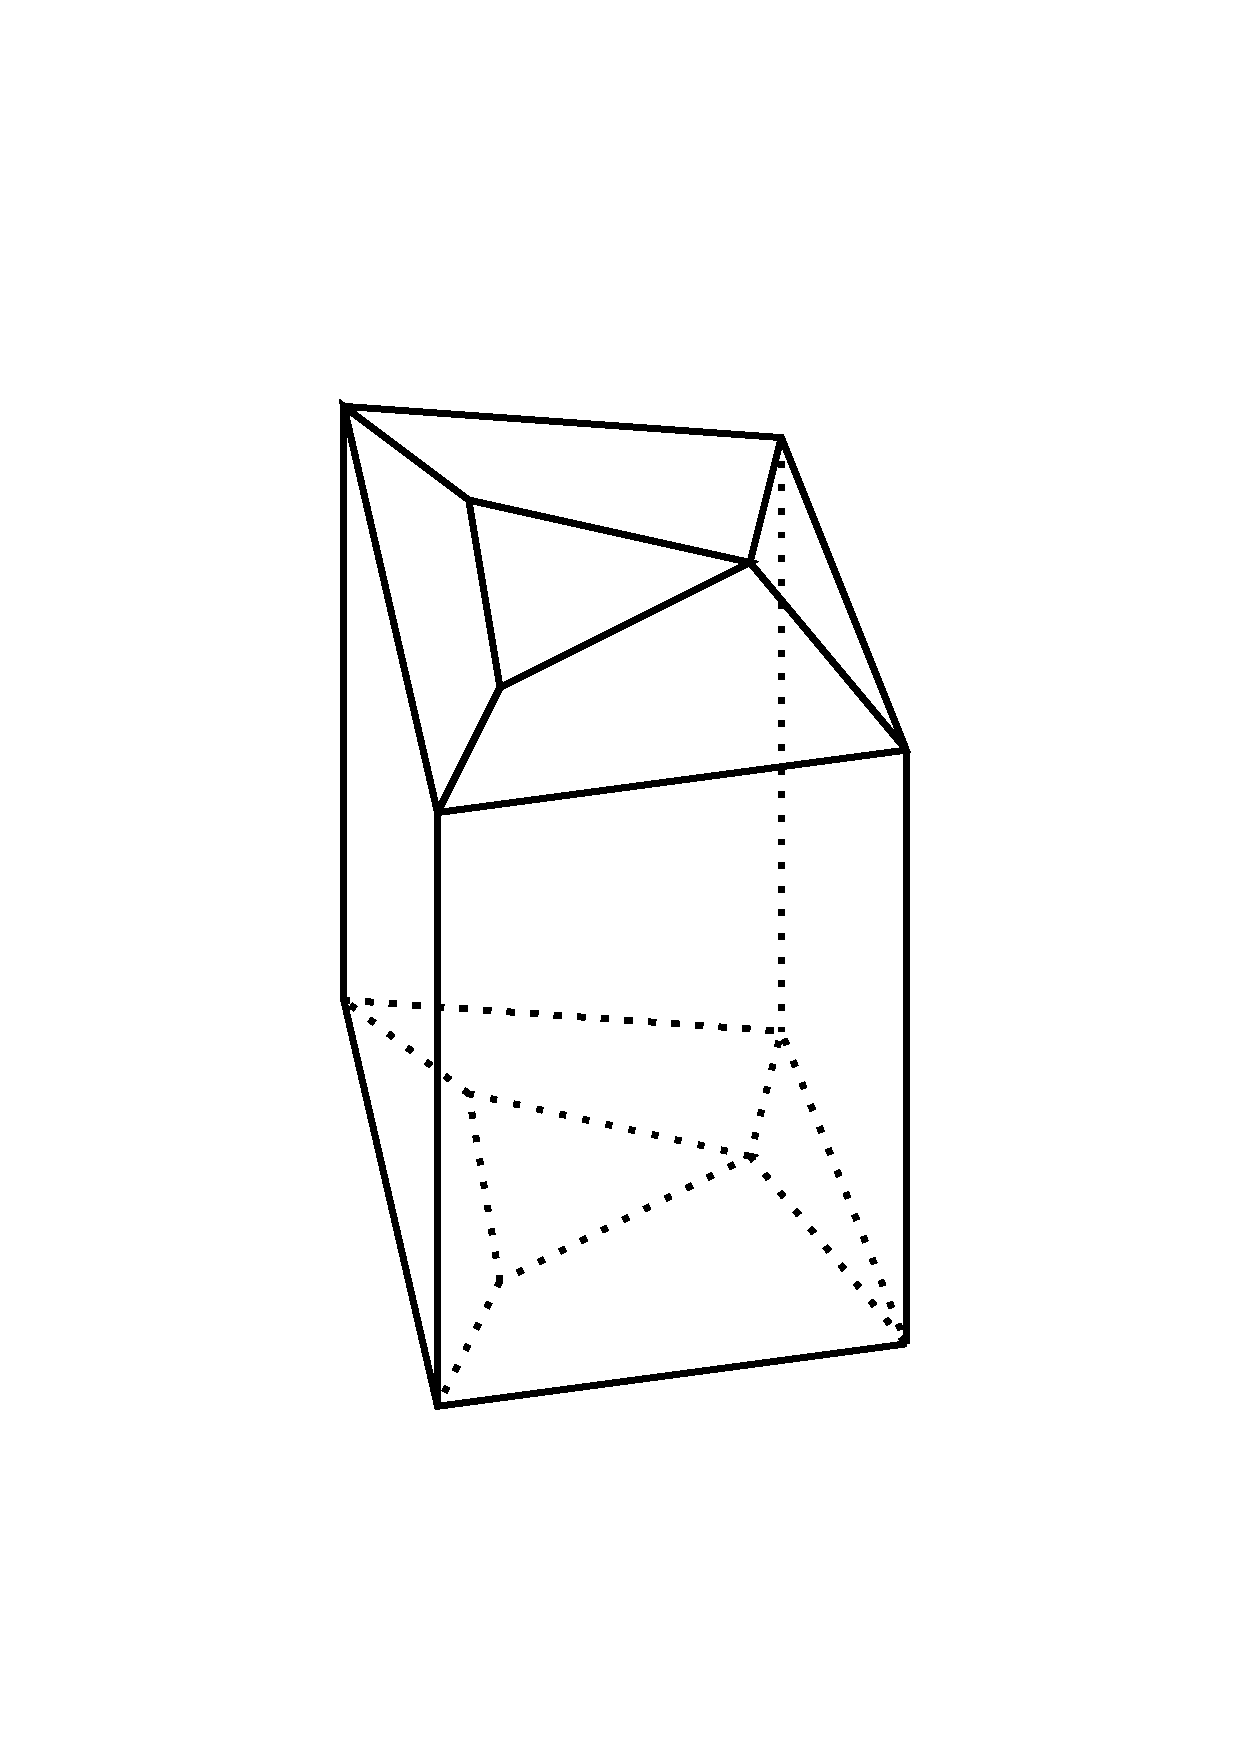
\includegraphics[width=\textwidth]{genus/genus-1}
        \caption{Genus zero.}
          \label{fig:initial-sphere}
        \end{subfigure}
          \hspace{.5cm}
         \begin{subfigure}[b]{0.2\textwidth}
        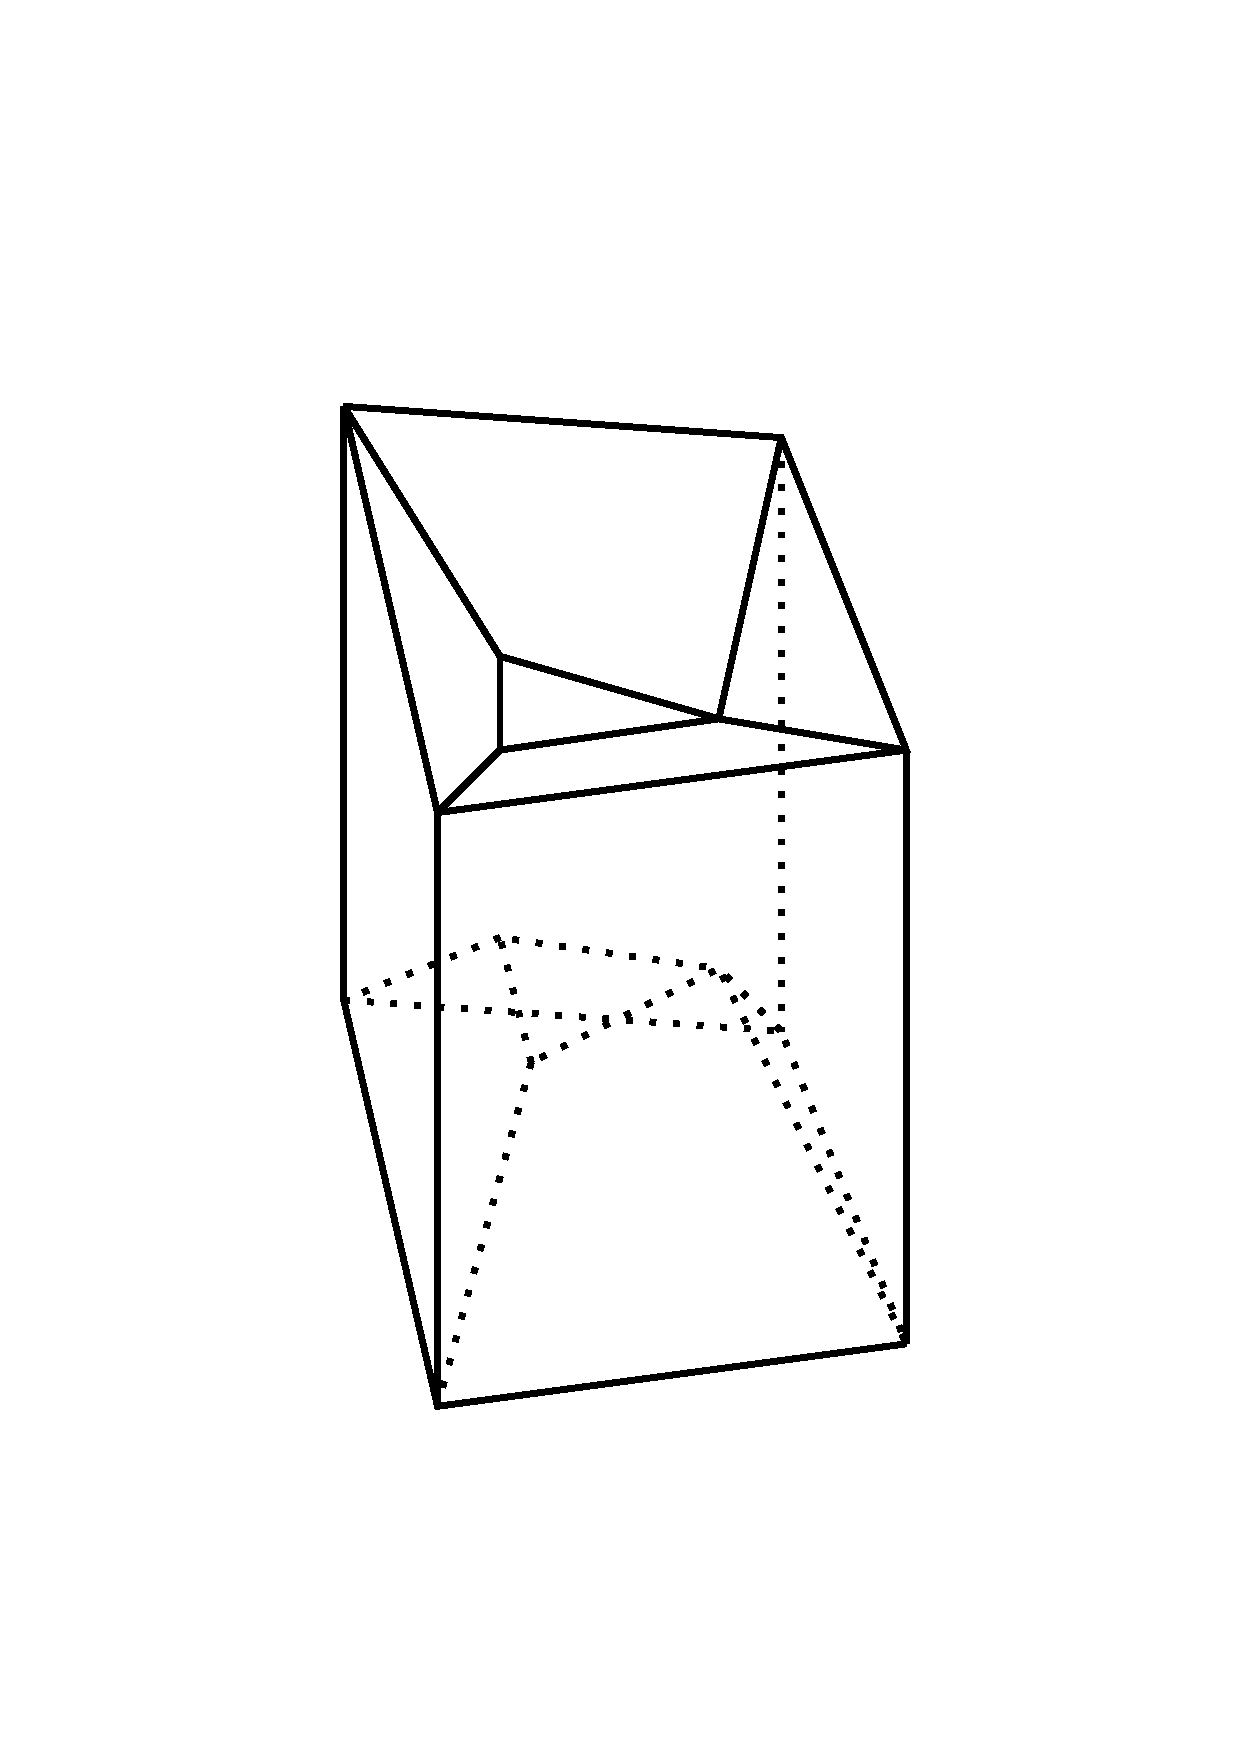
\includegraphics[width=\textwidth]{genus/genus-2}
        \caption{Deform.}
        \label{fig:decending-faces}
        \end{subfigure}
          \hspace{.5cm}
         \begin{subfigure}[b]{0.2\textwidth}
        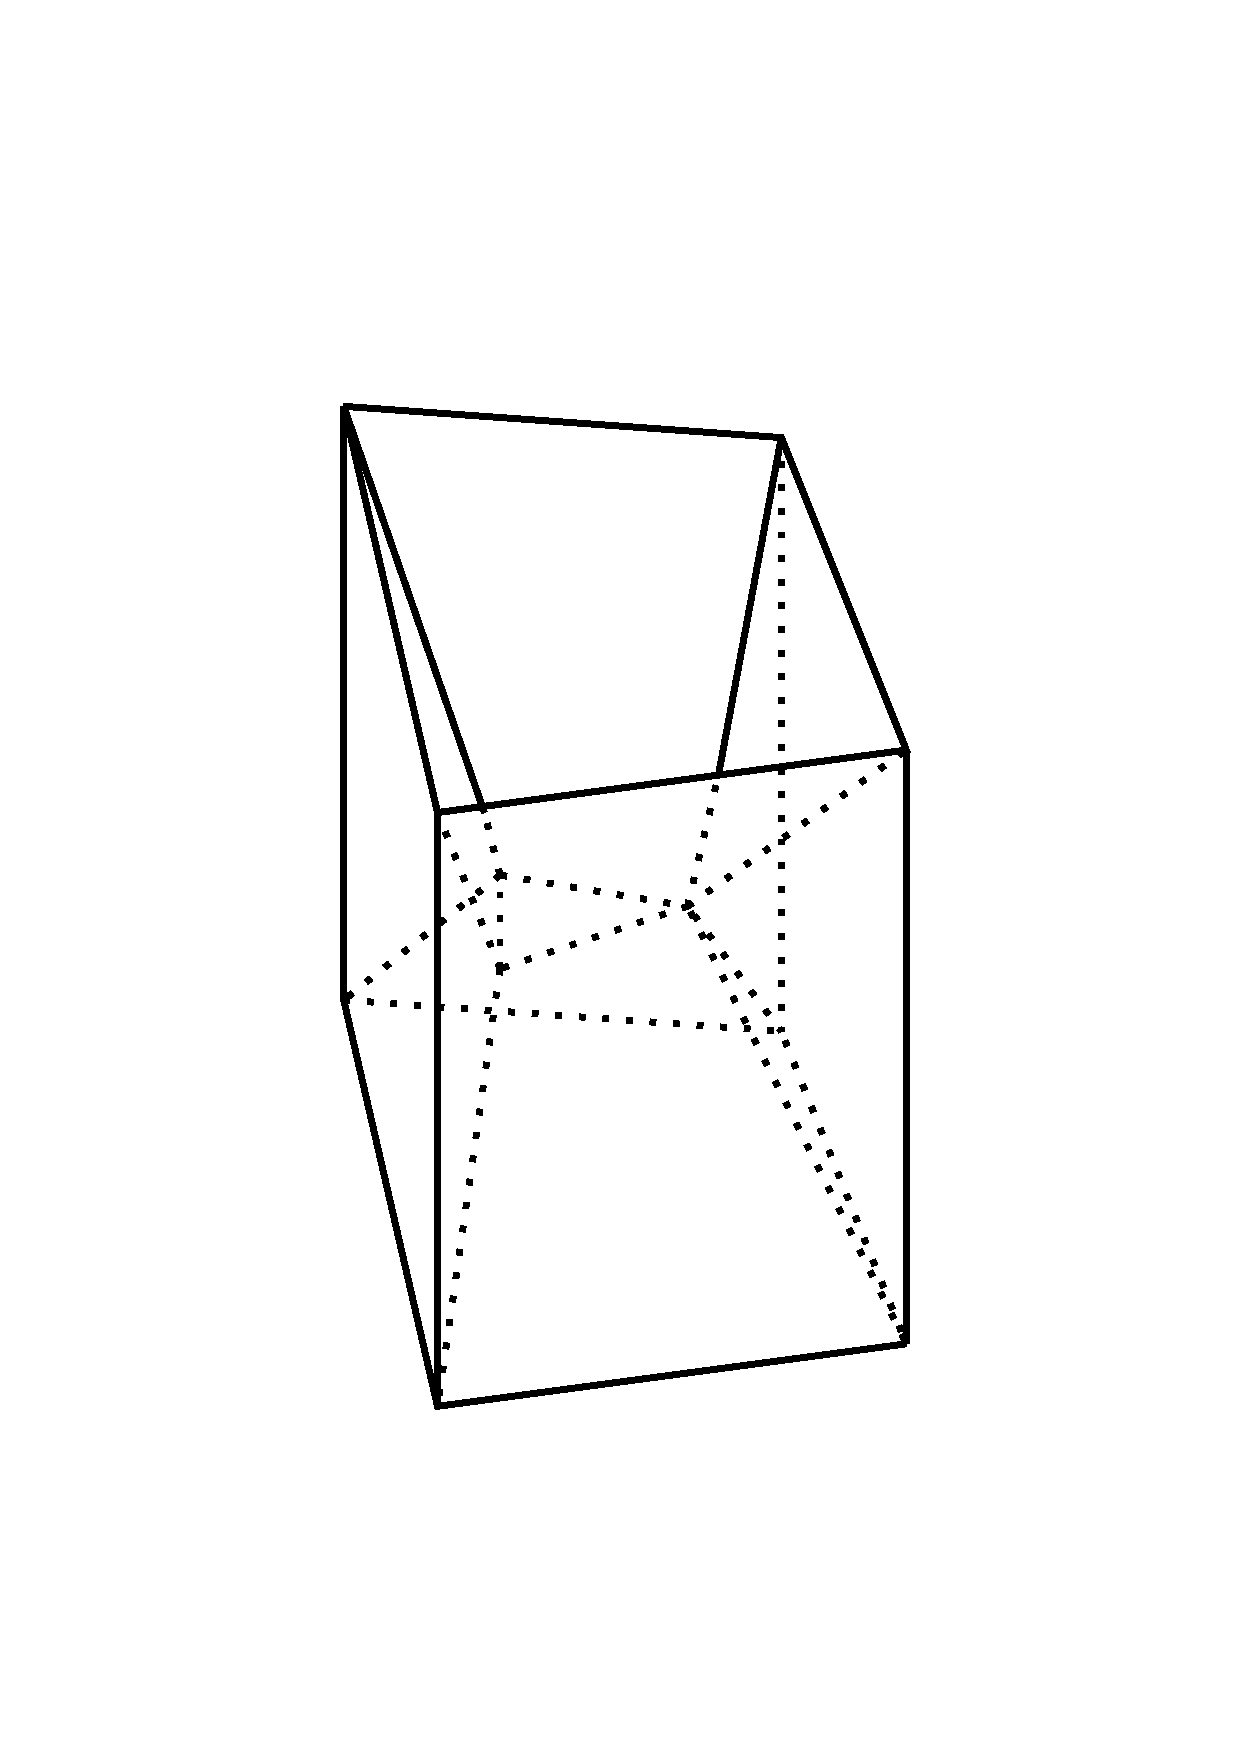
\includegraphics[width=\textwidth]{genus/genus-3}
        \caption{Triangles join.}
        \label{fig:faces-join}
        \end{subfigure}
		\caption{(\subref{fig:initial-sphere}) A surface homeomorphic to the sphere with genus zero.
		(\subref{fig:decending-faces}) The triangle on the top and the triangle on the bottom are getting
		closer. (\subref{fig:faces-join})  A surface homeomorphic to the torus. The triangle on the top
		and the triangle on the bottom have been removed. Three vertices and three edges are				removed. The Euler characteristic decreased by two.
		\label{fig:genus}}
\end{figure}

\noindent \textbf{Exercises}


\begin{enumerate}
	\item Given a mesh stored in a DCEL, give an pseudocode for an algorithm to iterate over all edges incident to a given vertex.
	
	\item Run a CGAL program on you local machine.
	
	\item How would you determine if two faces in a mesh intersect? Based on this, what is the runtime of \algref{self-intersection}?
	
\end{enumerate}

\pagebreak